\section{}
\label{sec:problem2}

%%%%%%%%%%%%%%%%%%%%%%%%%%%%%%%%%%%%%%%%%%%%%%%%%%%%%%%%%%%%%%%%%%%%%%
\paragraph{a)}
An area of size $(300 \times 300) \, \si{\meter^2}$ containing a pine tree forest is considered, and the actual locations of the pine trees are to be assessed. The pine tree locations are observed from a satellite by remote sensing, and due to partly cloudy weather the observation probability for individual trees vary across the area.

The area is discretized into a regular $(30 \times 30)$-grid $L$ with grid unit size $\SI{100}{\meter^2}$. The true, but unknown, number of pine trees located in each grid unit is \newline $\{k(\vect{x}) \ssep \vect{x} \in L\}$. The observed number of pine trees is shown in Figure~\ref{fig:p2_pines}. The probabilities for observing a pine tree in each grid unit is represented by $\{\alpha(\vect{x}) \ssep \vect{x} \in L\}$, see Figure~\ref{fig:p2_alpha}. There could seem to be more trees as $x$ and $y$ grows, but the observation probabilities also increase in the same direction. I.e. the random field might truly be stationary.

\begin{figure}
    \centering
    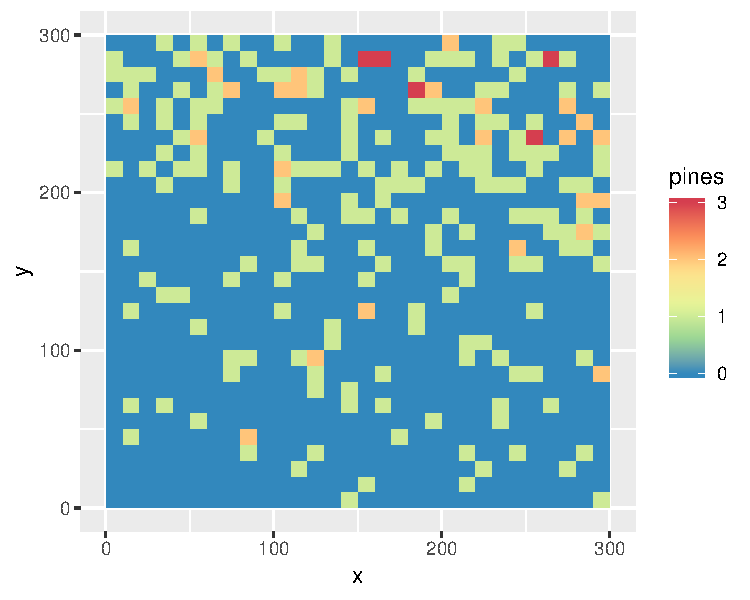
\includegraphics{figures/p2_pines.pdf}
    \caption{Plot of the number of observed pine trees in the grid defined in \ref{sec:problem2}a.}
    \label{fig:p2_pines}
\end{figure}

\begin{figure}
    \centering
    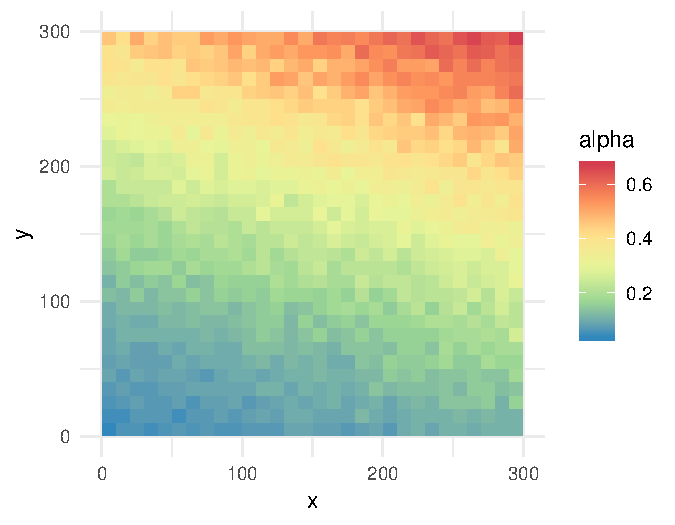
\includegraphics{figures/p2_alpha.pdf}
    \caption{Plot of the observation probabilities (of pine trees) in the grid defined in \ref{sec:problem2}a.}
    \label{fig:p2_alpha}
\end{figure}

Let $\vect{k}$ be the vector of the true number of pine trees per grid node, such that e.g. element 5 of $\vect{k}$, $k_5$, is the number of trees in the grid node centered at $(x, y) = (45, 5)$. Let, similarly, $\vect{d}$ be the vector of observations, i.e. the number of pine trees observed in each grid node, and $\vect{\alpha}$ be the vector of observation probabilities.

The number of observed pine trees in node $i$, $d_i$, is binomial with probability $\alpha_i$ and $n = k_i$. Assuming that the observations given the true number of pine trees are spatially uncorrelated from one grid unit to another, the likelihood $\lik$ for the observations is
%
\begin{equation*}
    \lik(\vect{k} \given{\vect{d}}) = \prod_{i=1}^n \binom{k_i}{d_i} \alpha_i^{d_i} (1 - \alpha_i)^{k_i - d_i} \, ,
\end{equation*}
%
where $n$ now equals 900, i.e. the number of grid nodes.

%%%%%%%%%%%%%%%%%%%%%%%%%%%%%%%%%%%%%%%%%%%%%%%%%%%%%%%%%%%%%%%%%%%%%%
\paragraph{b)}
We assume a priori that the distribution of pine trees is according to a stationary Poisson RF with model parameter $\lambda_k$. The expression for corresponding prior model for the discretized Poisson count model is
%
\begin{equation*}
    \prob(\vect{k} \given \lambda_k) = \prod_{i=1}^n \prob(k_i \given \lambda_k) = \prod_{i=1}^n \frac{(100\lambda_k)^{k_i} e^{-100\lambda_k}}{k_i!} = \frac{(100\lambda_k)^{\sum_{i=1}^n k_i} e^{-90000\lambda_k}}{\prod_{i=1}^n k_i!} \, .
\end{equation*}


%%%%%%%%%%%%%%%%%%%%%%%%%%%%%%%%%%%%%%%%%%%%%%%%%%%%%%%%%%%%%%%%%%%%%%
\paragraph{c)}
We wish to estimate the intensity $\lambda_k$ based on the observations and observation probabilities. An estimate of the total number of trees on the grid i $\sum_{i=1}^n d_i / \alpha_i$, and so an estimate of $\lambda_k$ is
%
\begin{equation*}
    \hat{\lambda_k} = \frac{\sum_{i=1}^n d_i / \alpha_i}{n} \approx 0.01016 \, .
\end{equation*}
%
There are (at least) two equivalent ways to simulate event counts and approximate event locations from the Poisson random field on $L$ with intensity $\hat{\lambda}$. One is to simulate from a Poisson distribution with parameter $|L|\hat{\lambda} = 90000\hat{\lambda}$ to get a total count $m$ and uniformly distribute the $m$ points over the grid. The other way is to simulate 900 times from a Poisson distribution with intensity $100\hat{\lambda}$ to get a vector of counts $\vect{m}$ corresponding to the 900 grid nodes. These are equivalent since we assume the field is stationary.

We do the latter for simplicity (when programming). The results are displayed in Figure~\ref{fig:p2_prior_sims}.

\begin{figure}
    \centering
    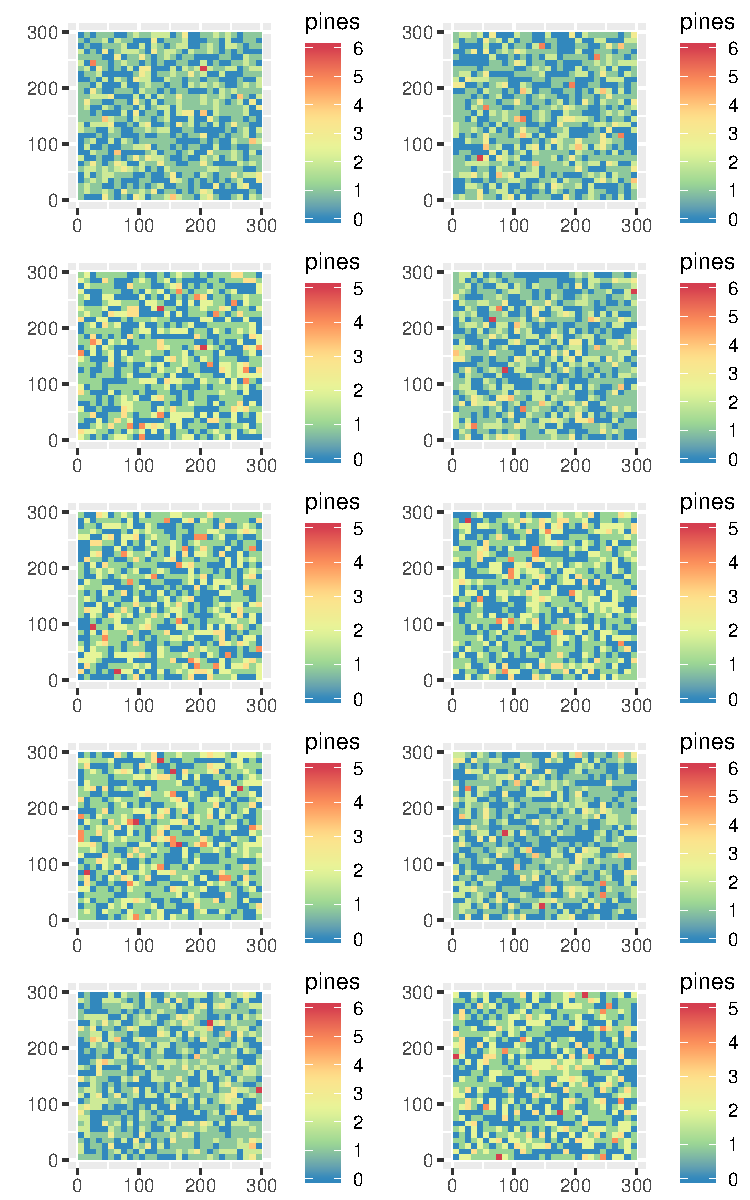
\includegraphics{figures/p2_prior_sims.pdf}
    \caption{10 realizations from the prior model defined in \ref{sec:problem2}b, i.e. we assume a stationary Poisson random field with intensity $\hat{\lambda}$ given in \ref{sec:problem2}c.}
    \label{fig:p2_prior_sims}
\end{figure}

%%%%%%%%%%%%%%%%%%%%%%%%%%%%%%%%%%%%%%%%%%%%%%%%%%%%%%%%%%%%%%%%%%%%%%
\paragraph{d)}
The posterior discretized  event-count model is given by
%
\begin{equation}
\label{eq:p2_posterior}
\begin{split}
    \prob(\vect{k} \given \vect{d}, \lambda_k) &\propto \prob(\vect{d} \given \vect{k}) \prob(k \given \lambda_k) \\
    &= \prod_{i=1}^n \frac{k_i!}{(k_i - d_i)!d_i!} \alpha_i^{d_i} (1 - \alpha_i)^{k_i - d_i} \prod_{i=1}^n \frac{(100\lambda_k)^{k_i} e^{-100\lambda_k}}{k_i!} \\
    &\propto \prod_{i=1}^n \frac{(100\lambda_k)^{k_i} e^{-100\lambda_k}}{(k_i - d_i)!} \alpha_i^{d_i} (1 - \alpha_i)^{k_i - d_i} \cdot \frac{(100\lambda_k)^{-d_i} e^{100\lambda_k\alpha_i}}{\alpha_i^{d_i}} \\
    &= \prod_{i=1}^n \frac{[100\lambda_k(1-\alpha_i)]^{k_i-d_i} e^{-[100\lambda_k(1-\alpha_i)]}}{(k_i-d_i)!} \, .
\end{split}
\end{equation}
%
By independence, the density of $k_i$, $i = 1, \dots, 900$, is given by removing the product symbol in the last line of \eqref{eq:p2_posterior}. I.e. $(k_i \given d_i, \lambda_k) \sim \Pois(k_i - d_i \ssep 100\lambda_k[1-\alpha_i])$. This makes sense intuitively; $\E(k_i - d_i \given d_i, \lambda_k) = 100\lambda_k(1-\alpha_i) = \E(k_i) - \alpha_i\E(k_i)$, i.e. the expected difference between $k_i$ and $d_i$ is just the expected number of pine trees, less the observation probability multiplied by the expected number of trees. Thus the posterior model is a Poisson RF model.

10 realizations of the associated approximate event-location model are generated in a similar way as in c). We simulate from the 900 Poisson distributions with intensities $100\lambda_k(1-\alpha_i)$ and add $d_i$, $i = 1, \dots, 900$. The results are illustrated in Figure~\ref{fig:p2_posterior_sims}.

\begin{figure}
    \centering
    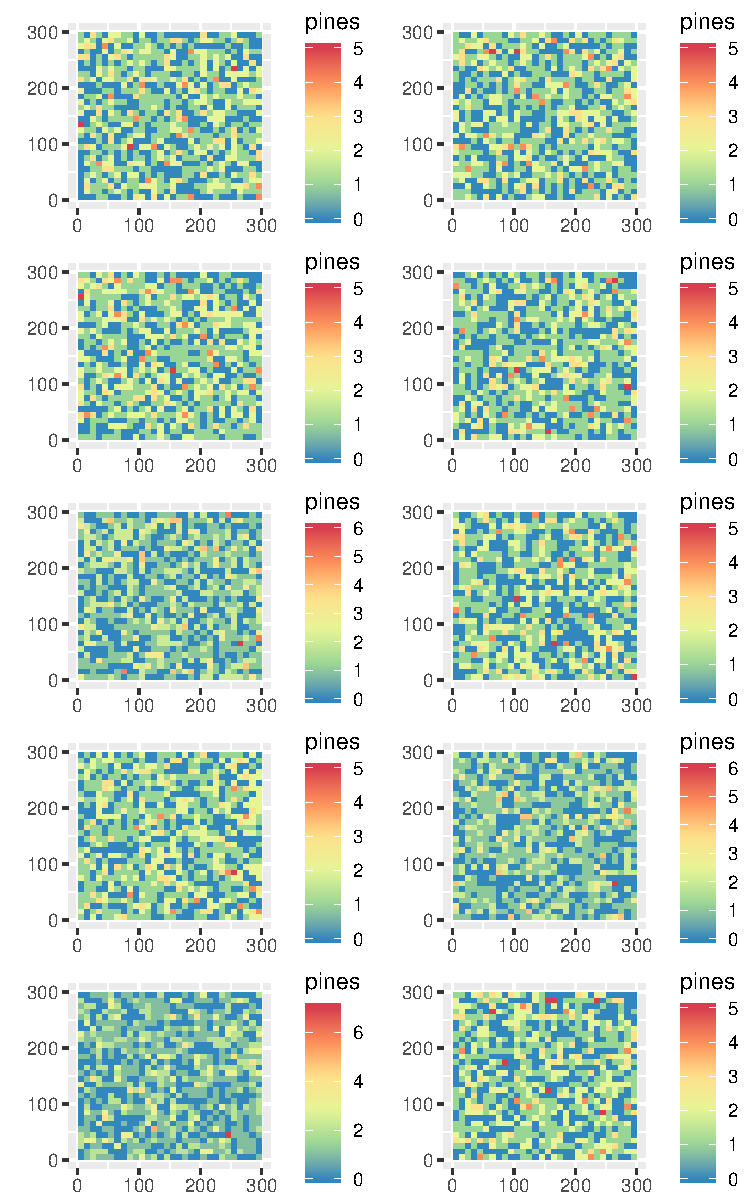
\includegraphics{figures/p2_posterior_sims.pdf}
    \caption{Plots of 10 realizations from the posterior model defined in \ref{sec:problem2}d with observation data $\vect{d}$ added.}
    \label{fig:p2_posterior_sims}
\end{figure}

Qualitatively there does not seem to be much of a difference between the prior and the posterior realizations. Looking closely one can see that in the posterior realizations (with observations $\vect{d}$ added), the points where trees are observed always have a at least the observed value - obviously. There don't seem to be any indications that the random field is not truly stationary, however. If we didn't add $\vect{d}$, the plots would indicate more pine trees towards low $x$ and $y$ values. This is simply because it is more likely that there are unobserved trees in that area.

Figure~\ref{fig:p2_posterior_mean} shows a plot of the posterior mean with $\vect{d}$ added. This illustrates the same points discussed in the previous paragraph; in short we know more about the number of trees in the area with higher observation probabilities.

\begin{figure}
    \centering
    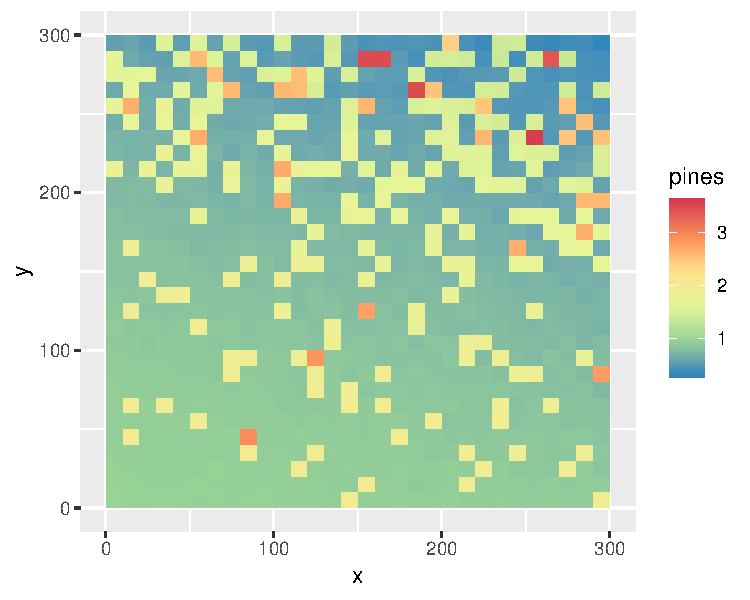
\includegraphics{figures/p2_posterior_mean.pdf}
    \caption{Posterior mean of the model defined in \ref{sec:problem2}d with observation data $\vect{d}$ added.}
    \label{fig:p2_posterior_mean}
\end{figure}
